\chapter{Specifikacija programske potpore}

\section{Funkcionalni zahtjevi}




\noindent \textbf{Dionici:}

\begin{packed_enum}

	\item Organizator (naručitelj)
	\item Sudionici kampa
	\item Animatori u kampu
	\item Razvojni tim

\end{packed_enum}
\vspace{10mm} %10mm vertical space
\noindent \textbf{Aktori i njihovi funkcionalni zahtjevi:}


\begin{packed_enum}
	\item  \underbar{Neregistrirani/neprijavljeni korisnik (inicijator) može:}

	\begin{packed_enum}

		\item pregledati osnovne informacije o kampu
		\begin{enumerate}
			\item vrijeme održavanja
			\item mjesto održavanja
			\item kratak opis
			\item kontakt organizatora
			\item popis aktivnosti
		\end{enumerate}
		\item prijaviti se na kamp kao sudionik ili kao animator

	\end{packed_enum}
\vspace{10mm} %10mm vertical space

	\item  \underbar{Sudionik može: }

	\begin{packed_enum}

		\item pregledavati i mijenjati osobne podatke
		\item izbrisati svoj korisnički račun
		\item vidjeti svoj raspored aktivnosti
		\item vidjeti informacije o grupi u koju je dodijeljen
		\item vidjeti kontakt podatke o animatoru koji je zadužen za njegovu grupu
		\item imati uvid u popis odrađenih aktivnosti
		\item ocijeniti sve aktivnosti koje je odradio ocjenama od 1 do 10
		\item dati ocjenu cjelokupnog dojma po završetku kampa

	\end{packed_enum}
	\vspace{5mm} %5mm vertical space

	\item  \underbar{Animator može:}

	\begin{packed_enum}

		\item vidjeti raspored aktivnosti koje je dužan predvoditi
		\item vidjeti popis svih grupa u kampu
		\item vidjeti popis i informacije o svim sudionicima u kampu
		\item vidjeti popis svih aktivnosti koje je odradio
		\item ocijeniti sve aktivnosti koje je odradio ocjenama od 1 do 10

	\end{packed_enum}
	\vspace{5mm} %5mm vertical space

	\item  \underbar{Organizator može:}

	\begin{packed_enum}

		\item odrediti vrijeme početka kampa
		\item vidjeti popis svih registriranih korisnika i njihovih osobnih podataka
		\item odbiti ili prihvatiti zaprimljene prijave od strane korisnika
		\item odrediti broj grupa u koje će se rasporediti sudionici
		\item mijenjati pripadnost grupi proizvoljnih sudionika
		\item popuniti raspored aktivnostima u kojima sudjeluju grupe i animatori (pri tome paziti na pravila o preklapanju aktivnosti)
		\item vidjeti popi ocjena za svaku aktivnost na kojoj su sudjelovali sudionici i animatori

	\end{packed_enum}
	\vspace{5mm} %5mm vertical space

	\item  \underbar{Baza podataka (sudionik):}

	\begin{packed_enum}

		\item pohranjuje sve podatke o korisnicima
		\item pohranjuje sve podatke i razinama ovlasti korisnika
		\item pohranjuje sve podatke vezane uz sadržaje kampa (raspored, aktivnosti, grupe)

	\end{packed_enum}
\end{packed_enum}



\eject



\subsection{Obrasci uporabe}
	\vspace{10mm} %10mm vertical space




\noindent \underbar{\textbf{UC1 -Početna stranica}}
\begin{packed_item}

	\item \textbf{Glavni sudionik: }Sudionici i animatori
	\item  \textbf{Cilj:} Pregledati informacije o kampu te se po mogućnosti prijaviti
	\item  \textbf{Sudionici:} Baza podataka
	\item  \textbf{Preduvjet:} -
	\item  \textbf{Opis osnovnog tijeka:}

	\item[] \begin{packed_enum}

				\item Korisnik na stranici vidi osnovne informacije o kampu
				\item U slučaju zainteresiranosti, korisnik ima mogućnost kliknuti gumb za stvaranje računa kao sudionik ili animator

	\end{packed_enum}

\end{packed_item}
\vspace{5mm} %5mm vertical space

\noindent \underbar{\textbf{UC2 -Registracija}}
\begin{packed_item}

	\item \textbf{Glavni sudionik: }Sudionici i animatori
	\item  \textbf{Cilj:} Stvoriti korisnički račun za pristup sustavu
	\item  \textbf{Sudionici:} Baza podataka
	\item  \textbf{Preduvjet:} -
	\item  \textbf{Opis osnovnog tijeka:}

	\item[] \begin{packed_enum}

				\item Korisnik odabire opciju za registraciju
				\item Korisnik unosi potrebne korisničke podatke
				\item Korisnik prima obavijest u obliku emaila o uspješnoj registraciji
				\item Klikom na link u mailu korisnik odabire šifru za svoj račun u sustavu
	\end{packed_enum}

	\item  \textbf{Opis mogućih odstupanja:}

	\begin{packed_item}


		\item[2.a] Odabir već zauzetog korisničkog imena i/ili e-maila, unos korisničkog podatka u
		\begin{enumerate}
			\item Sustav obavještava korisnika o neuspjelom upisu i vraća ga na stranicu za registraciju
			\item Korisnik mijenja potrebne podatke te završava unos ili odustaje od registracije


		\end{enumerate}
	\end{packed_item}
\end{packed_item}
\pagebreak
\noindent \underbar{\textbf{UC3 -Prijava u sustav (prije početka kampa)}}
\begin{packed_item}

	\item \textbf{Glavni sudionik: }Sudionici i animatori
	\item  \textbf{Cilj:} Dobiti informaciju o početku kampa (odbrojavanje u određenom vremenskom formatu)
	\item  \textbf{Sudionici:} -
	\item  \textbf{Preduvjet:} Registracija
	\item  \textbf{Opis osnovnog tijeka:}

	\item[] \begin{packed_enum}

				\item Unos korisničkog imena i lozinke
				\item Potvrda o ispravnosti unesenih podataka
				\item Pristup satu za odbrojavanje
	\end{packed_enum}

	\item  \textbf{Opis mogućih odstupanja:}

	\item[] \begin{packed_item}

				\item[2.a] Neispravno korisničko ime ili lozinka
				\item[] \begin{packed_enum}

							\item Sustav obavještava korisnika o neuspjelom upisu i vraća ga na stranicu za registraciju


				\end{packed_enum}

	\end{packed_item}
\end{packed_item}
	
\vspace{5mm} %5mm vertical space
\noindent \underbar{\textbf{UC4 -Odabir lozinke}}
\begin{packed_item}

	\item \textbf{Glavni sudionik: }Sudionici i animatori
	\item  \textbf{Cilj:} Odabrati lozinku koja će korisniku služiti za prijavu u sustav
	\item  \textbf{Sudionici:} Baza podataka
	\item  \textbf{Preduvjet:} Registracija
	\item  \textbf{Opis osnovnog tijeka:}

	\item[] \begin{packed_enum}

				\item Unos željene lozinke
				\item Potvrda o uspješnom stvaranju korisničkog računa u bazi podataka
	\end{packed_enum}

	\item  \textbf{Opis mogućih odstupanja:}

	\item[] \begin{packed_item}

				\item[2.a] Ne unošenje lozinke u predviđeni prostor te izlazak iz web aplikacije
				\item[] \begin{packed_enum}

							\item Sustav odbacuje prijavu

				\end{packed_enum}


	\end{packed_item}
\end{packed_item}
\vspace{5mm} %5mm vertical space

\noindent \underbar{\textbf{UC5 -Prijava u sustav (nakon početka kampa) - sudionici}}
\begin{packed_item}

	\item \textbf{Glavni sudionik: }Sudionici i animatori
	\item  \textbf{Cilj:} Pregled korisničkog sučelja koje se sastoji od rasporeda aktivnosti,                 informacijama o dodijeljenoj grupi i animatoru te popisu odrađenih aktivnosti
	\item  \textbf{Sudionici:} Baza podataka
	\item  \textbf{Preduvjet:} Registracija
	\item  \textbf{Opis osnovnog tijeka:}

	\item[] \begin{packed_enum}

				\item Unos korisničkog imena i lozinke
				\item Potvrda o ispravnosti unesenih podataka
				\item Pristup rasporedu aktivnosti te informacijama o dodijeljenoj grupi i animatoru
	\end{packed_enum}

	\item  \textbf{Opis mogućih odstupanja:}

	\item[] \begin{packed_item}

				\item[2.a] Neispravno korisničko ime ili lozinka
				\item[] \begin{packed_enum}

							\item Sustav obavještava korisnika o neuspjelom upisu i vraća ga na stranicu za registraciju


				\end{packed_enum}
	\end{packed_item}
\end{packed_item}
\vspace{5mm} %5mm vertical space

\noindent \underbar{\textbf{UC6 -Prijava u sustav (nakon početka kampa) - animatori}}
\begin{packed_item}

	\item \textbf{Glavni sudionik: }Sudionici i animatori
	\item  \textbf{Cilj:} Pregled korisničkog sučelja koje se sastoji od rasporeda aktivnosti, informacijama o svim grupama i sudionicima kampa te popisu odrađenih aktivnosti
	\item  \textbf{Sudionici:} Baza podataka
	\item  \textbf{Preduvjet:} Registracija
	\item  \textbf{Opis osnovnog tijeka:}

	\item[] \begin{packed_enum}

				\item Unos korisničkog imena i lozinke
				\item Potvrda o ispravnosti unesenih podataka
				\item Pristup informacijama o svim grupama i sudionicima kampa
	\end{packed_enum}

	\item  \textbf{Opis mogućih odstupanja:}

	\item[] \begin{packed_item}

				\item[2.a] Neispravno korisničko ime ili lozinka
				\item[] \begin{packed_enum}

							\item Sustav obavještava korisnika o neuspjelom upisu i vraća ga na stranicu za registraciju
				\end{packed_enum}

	\end{packed_item}
\end{packed_item}
\vspace{5mm} %5mm vertical space

\noindent \underbar{\textbf{UC7 -Pregled osobnih podataka}}
\begin{packed_item}

	\item \textbf{Glavni sudionik: }Sudionici i animatori
	\item  \textbf{Cilj:} Pregledati osobne podatke
	\item  \textbf{Sudionici:} Baza podataka
	\item  \textbf{Preduvjet:} Klijent je prijavljen
	\item  \textbf{Opis osnovnog tijeka:}

	\item[] \begin{packed_enum}

				\item Korisnik odabire opciju ”Osobni podatci”
				\item Aplikacija prikazuje osobne podatke korisnika
	\end{packed_enum}



\end{packed_item}
\pagebreak
\vspace{5mm} %5mm vertical space

\noindent \underbar{\textbf{UC8 -Promjena osobnih podataka}}
\begin{packed_item}

	\item \textbf{Glavni sudionik: }Sudionici i animatori
	\item  \textbf{Cilj:} Promijeniti osobne podatke
	\item  \textbf{Sudionici:} Baza podataka
	\item  \textbf{Preduvjet:} Klijent je prijavljen
	\item  \textbf{Opis osnovnog tijeka:}

	\item[] \begin{packed_enum}

				\item Korisnik odabere opciju za promjenu podataka
				\item Korisnik mijenja svoje osobne podatke
				\item Korisnik sprema promjene
				\item Baza podataka se ažurira
	\end{packed_enum}

	\item  \textbf{Opis mogućih odstupanja:}

	\item[] \begin{packed_item}

				\item[2.a] Korisnik promijeni svoje osobne podatke, ali ne odabere opciju ”Spremi promjenu”
				\item[] \begin{packed_enum}

							\item Sustav obavještava korisnika da nije spremio podatke prije izlaska iz prozora


				\end{packed_enum}


	\end{packed_item}
\end{packed_item}

\vspace{5mm} %5mm vertical space

\noindent \underbar{\textbf{UC9 -Brisanje korisničkog računa}}
\begin{packed_item}

	\item \textbf{Glavni sudionik: }Sudionici i animatori
	\item  \textbf{Cilj:} Izbrisati svoj korisnički račun
	\item  \textbf{Sudionici:} Baza podataka
	\item  \textbf{Preduvjet:} Klijent je prijavljen
	\item  \textbf{Opis osnovnog tijeka:}

	\item[] \begin{packed_enum}

				\item Korisnik pregledava osobne podatke
				\item Otvara se stranica s osobnim podacima korisnika
				\item Korisnik briše račun
				\item Korisnički račun se briše iz baze podataka
				\item Otvara se stranica za registraciju
	\end{packed_enum}



\end{packed_item}
\vspace{5mm} %5mm vertical space

\noindent \underbar{\textbf{UC10 -Popis odrađenih aktivnosti}}
\begin{packed_item}

	\item \textbf{Glavni sudionik: }Sudionici i animatori
	\item  \textbf{Cilj:} Vidjeti popis odrađenih aktivnosti te ocijeniti ih ocjenom od 1 do 10
	\item  \textbf{Sudionici:} Baza podataka
	\item  \textbf{Preduvjet:} Klijent je prijavljen
	\item  \textbf{Opis osnovnog tijeka:}

	\item[] \begin{packed_enum}

				\item Klijent vidi popis svih odrađenih aktivnosti
				\item Klijent odabire aktivnost koju želi ocijeniti
				\item Klijent ocjenjuje aktivnost željenom ocjenom
				\item Klijent odabire opciju ”Ocijeni”, kojom završava proces ocjenjivanja
	\end{packed_enum}


\end{packed_item}
\vspace{5mm} %5mm vertical space

\noindent \underbar{\textbf{UC11 -Završetak kampa – sudionici i animatori}}
\begin{packed_item}

	\item \textbf{Glavni sudionik: }Sudionici i animatori
	\item  \textbf{Cilj:} Ocjena cjelokupnog dojma kampa
	\item  \textbf{Sudionici:} Klijent je prijavljen
	\item  \textbf{Preduvjet:} $<$preduvjet$>$
	\item  \textbf{Opis osnovnog tijeka:}

	\item[] \begin{packed_enum}

				\item Klijent ocjenjuje cjelokupan doživljaj na kampu
	\end{packed_enum}


\end{packed_item}
\vspace{5mm} %5mm vertical space

\noindent \underbar{\textbf{UC12 -Sučelje za organizatore}}
\begin{packed_item}

	\item \textbf{Glavni sudionik: }Organizator
	\item  \textbf{Cilj:} Uvid u sve operacije koje obavlja organizator za vrijeme i i nakon trajanja          kampa.
	\item  \textbf{Sudionici:} Baza podataka
	\item  \textbf{Preduvjet:} Organizator je prijavljen i kamp je započeo
	\item  \textbf{Opis osnovnog tijeka:}

	\item[] \begin{packed_enum}
				\item Unos korisničkog imena i lozinke
				\item Potvrda o ispravnosti unesenih podataka
				\item Pristup informacijama o svim grupama i sudionicima kampa
				\item Organizator se prijavljuje u sustav
				\item Prikaz gumbova i poveznica za sljedeće akcije:
				\begin{enumerate}
					\item Definiranje aktivnosti
					\item Uvid u zaprimljene prijave korisnika i sudionika
					\item Određivanje broja grupa
					\item Stvaranje rasporeda za korisnike i animatore
				\end{enumerate}
				\item Organizator odabire gumb ili akciju koju želi izvršiti, te odlazi na novu stranicu
	\end{packed_enum}


\end{packed_item}

\pagebreak
\noindent \underbar{\textbf{UC13 -Definiranje aktivnosti}}
\begin{packed_item}

	\item \textbf{Glavni sudionik: }Organizator
	\item  \textbf{Cilj:} Stvoriti novu aktivnost.
	\item  \textbf{Sudionici:} Baza podataka
	\item  \textbf{Preduvjet:} Organizator je prijavljen.
	\item  \textbf{Opis osnovnog tijeka:}

	\item[] \begin{packed_enum}

				\ \item Organizator vidi obrazac za stvaranje definiranje nove aktivnosti koji se            sastoji od sljedećih polja:
				\begin{enumerate}
					\item Ime aktivnosti
					\item Kratki opis
					\item Vremensko trajanje aktivnosti
					\item Tip aktivnosti (4 tipa s obzirom na broj grupa koje sudjeluju u kampu)
				\end{enumerate}
	\end{packed_enum}

	\item  \textbf{Opis mogućih odstupanja:}

	\item[] \begin{packed_item}

				\item[2.a] \item Organizator ne ispuni barem jedno od potrebnih polja za unos
				\item[] \begin{packed_enum}

							\item Vraćanje na sučelje za organizatore


				\end{packed_enum}


	\end{packed_item}
\end{packed_item}
\vspace{5mm} %5mm vertical space

\noindent \underbar{\textbf{UC14 -Prihvaćanje i odbijanje prijava}}
\begin{packed_item}

	\item \textbf{Glavni sudionik: }Organizator
	\item  \textbf{Cilj:} Prihvatiti ili odbiti prijave sudionika i animatora
	\item  \textbf{Sudionici:} Baza podataka
	\item  \textbf{Preduvjet:} Organizator je prijavljen i barem jedan korisnik je napravio prijavu
	\item  \textbf{Opis osnovnog tijeka:}

	\item[] \begin{packed_enum}

				\item Organizator odabire opciju uvida u prijave
				\item Prikazuje se lista svih prijava koje sadržavaju osobne podatke o korisnicima
				\item Prikaz dvaju gumbova, od kojih jedan služi za prihvaćanje prijave i stvaranje         korisničkog računa, dok drugi služi za odbijanje prijave

	\end{packed_enum}




\end{packed_item}
\pagebreak
\vspace{5mm} %5mm vertical space

\noindent \underbar{\textbf{UC15 -Određivanje broja grupa}}
\begin{packed_item}

	\item \textbf{Glavni sudionik: }Organizator
	\item  \textbf{Cilj:} Odrediti broj grupa u koje će sudionici biti raspodijeljeni.
	\item  \textbf{Sudionici:} Baza podataka
	\item  \textbf{Preduvjet:} \begin{packed_enum}


								   \item Organizator je prijavljen
								   \item Proces prijava korisnika za kamp je završio
	\end{packed_enum}
	\item  \textbf{Opis osnovnog tijeka:}

	\item[] \begin{packed_enum}

				\item Organizator vidi popis svih uspješno prijavljenih sudionika
				\item U polju za unos podatka o broju grupa unosi željeni broj grupa u brojčanom       obliku
				\begin{enumerate}
					\item 3.	Izvršava se automatska dodjela sudionika u grupe
				\end{enumerate}
	\end{packed_enum}

	\item  \textbf{Opis mogućih odstupanja:}

	\item[] \begin{packed_item}

				\item[2.a] Organizator u polje za unos napiše nešto što nije broj ili negativni broj
				\item[] \begin{packed_enum}

							\item Sustav javlja poruku o pogrešnom unosu te organizatora vraća na          stranicu za određivanje grupa (refresh)

				\end{packed_enum}
				\item[2.b]Organizator u polje za unos, unosi broj veći od broja svih sudionika
				\item[] \begin{packed_enum}

							\item	Sustav stvara broj grupa jednak broju sudionika, tako da svaki           korisnik čini jednu grupu, a ostali broj grupa zanemaruje.


				\end{packed_enum}



	\end{packed_item}
\end{packed_item}

\noindent \underbar{\textbf{UC16 -Kreiranje rasporeda}}
\begin{packed_item}

	\item \textbf{Glavni sudionik: }Organizator
	\item  \textbf{Cilj:} Stvoriti raspored koji će koristiti sudionici i animatori
	\item  \textbf{Sudionici:} Baza podataka
	\item  \textbf{Preduvjet:} Organizator je prijavljen i svi korisnici su prijavljeni u sustav
	\item  \textbf{Opis osnovnog tijeka:}

	\item[] \begin{packed_enum}

				\item Organizator odabire opciju stvaranja rasporeda
				\item Prikaz tjednog rasporeda po danima
				\item Organizator za svaku aktivnost određuje sljedeća svojstva:

				\begin{enumerate}
					\item Vrijeme održavanja
					\item Grupe koje prisustvuju aktivnosti
					\item Animator/e koji predvodi/e aktivnost
				\end{enumerate}
				\item Onemogućeno je dodavanje aktivnosti koje ne poštuju pravila o preklapanju u rasporedu

	\end{packed_enum}

	\item  \textbf{Opis mogućih odstupanja:}

	\item[] \begin{packed_item}

				\item[2.a] Organizator u polje za unos napiše nešto što nije broj ili negativni broj
				\item[] \begin{packed_enum}

							\item Sustav javlja poruku o pogrešnom unosu te organizatora vraća na          stranicu za određivanje grupa (refresh)



				\end{packed_enum}
				\item[2.b]Organizator u polje za unos, unosi broj veći od broja svih sudionika

				\item[] \begin{packed_enum}

							\item Sustav stvara broj grupa jednak broju sudionika, tako da svaki           korisnik čini jednu grupu, a ostali broj grupa zanemaruje.
				\end{packed_enum}
	\end{packed_item}
\end{packed_item}

\pagebreak

\subsubsection{Dijagrami obrazaca uporabe}
\begin{figure}[H]
	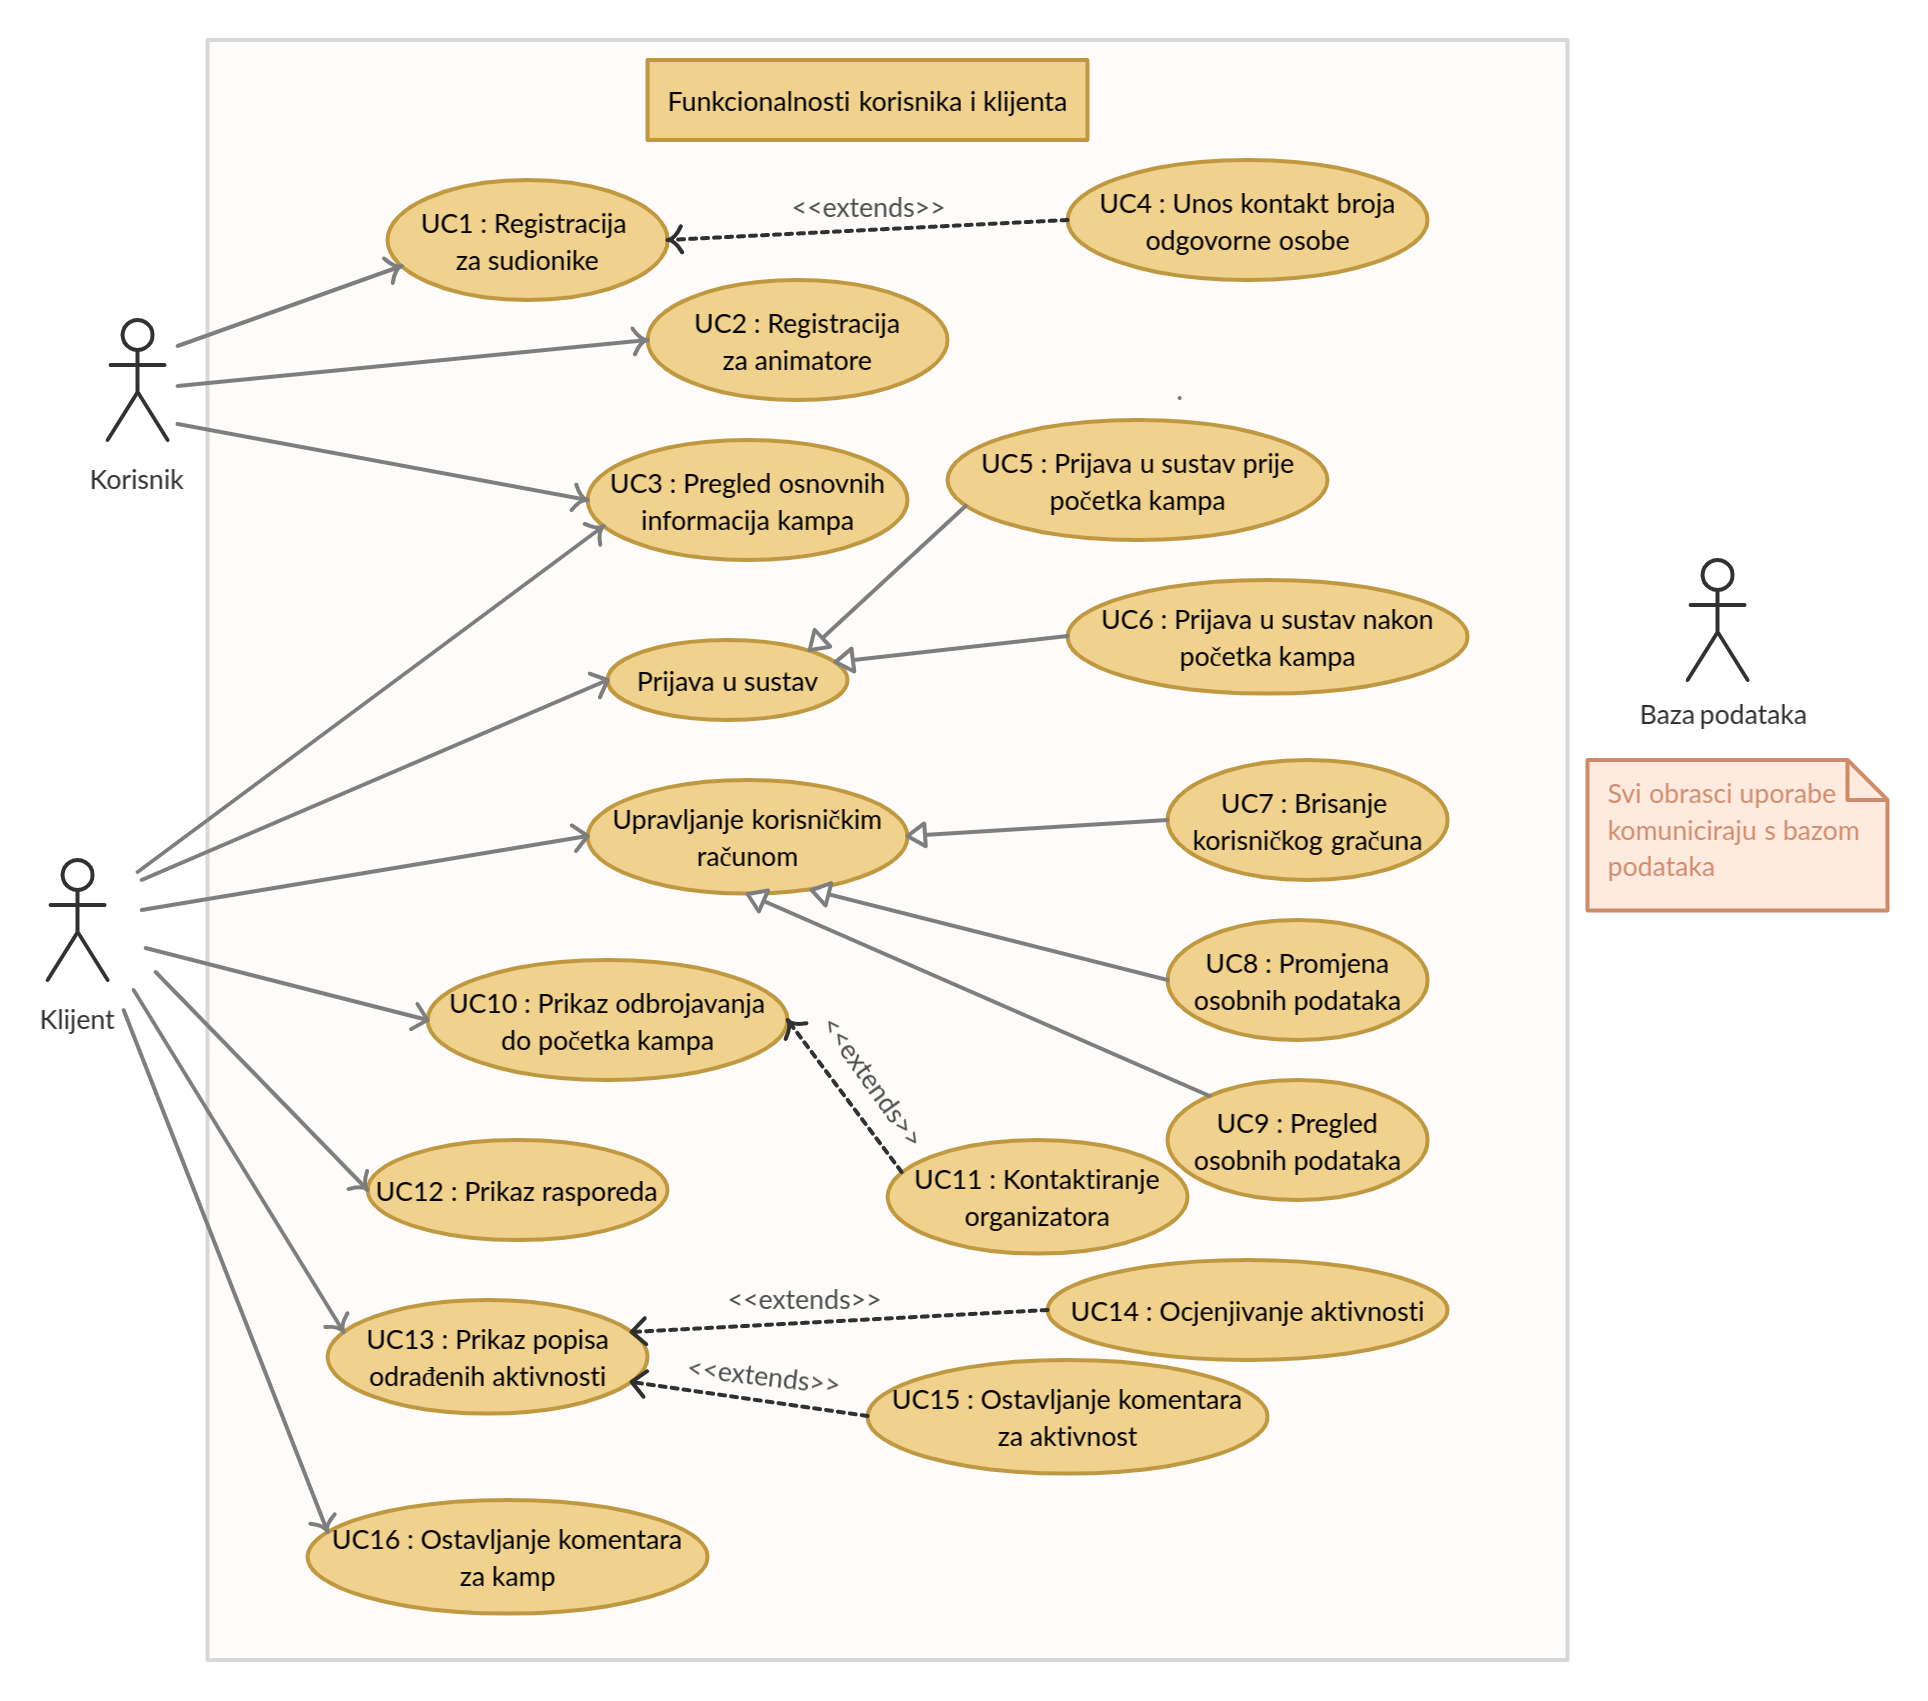
\includegraphics[scale=0.26]{dijagrami/Korisnik i klijent.jpg} %veličina slike u odnosu na originalnu datoteku i pozicija slike
	\centering
	\caption{Dijagram obrasca uporabe korisnik-klijent}
	\label{fig:promjene}
\end{figure}

\pagebreak

\begin{figure}[H]
	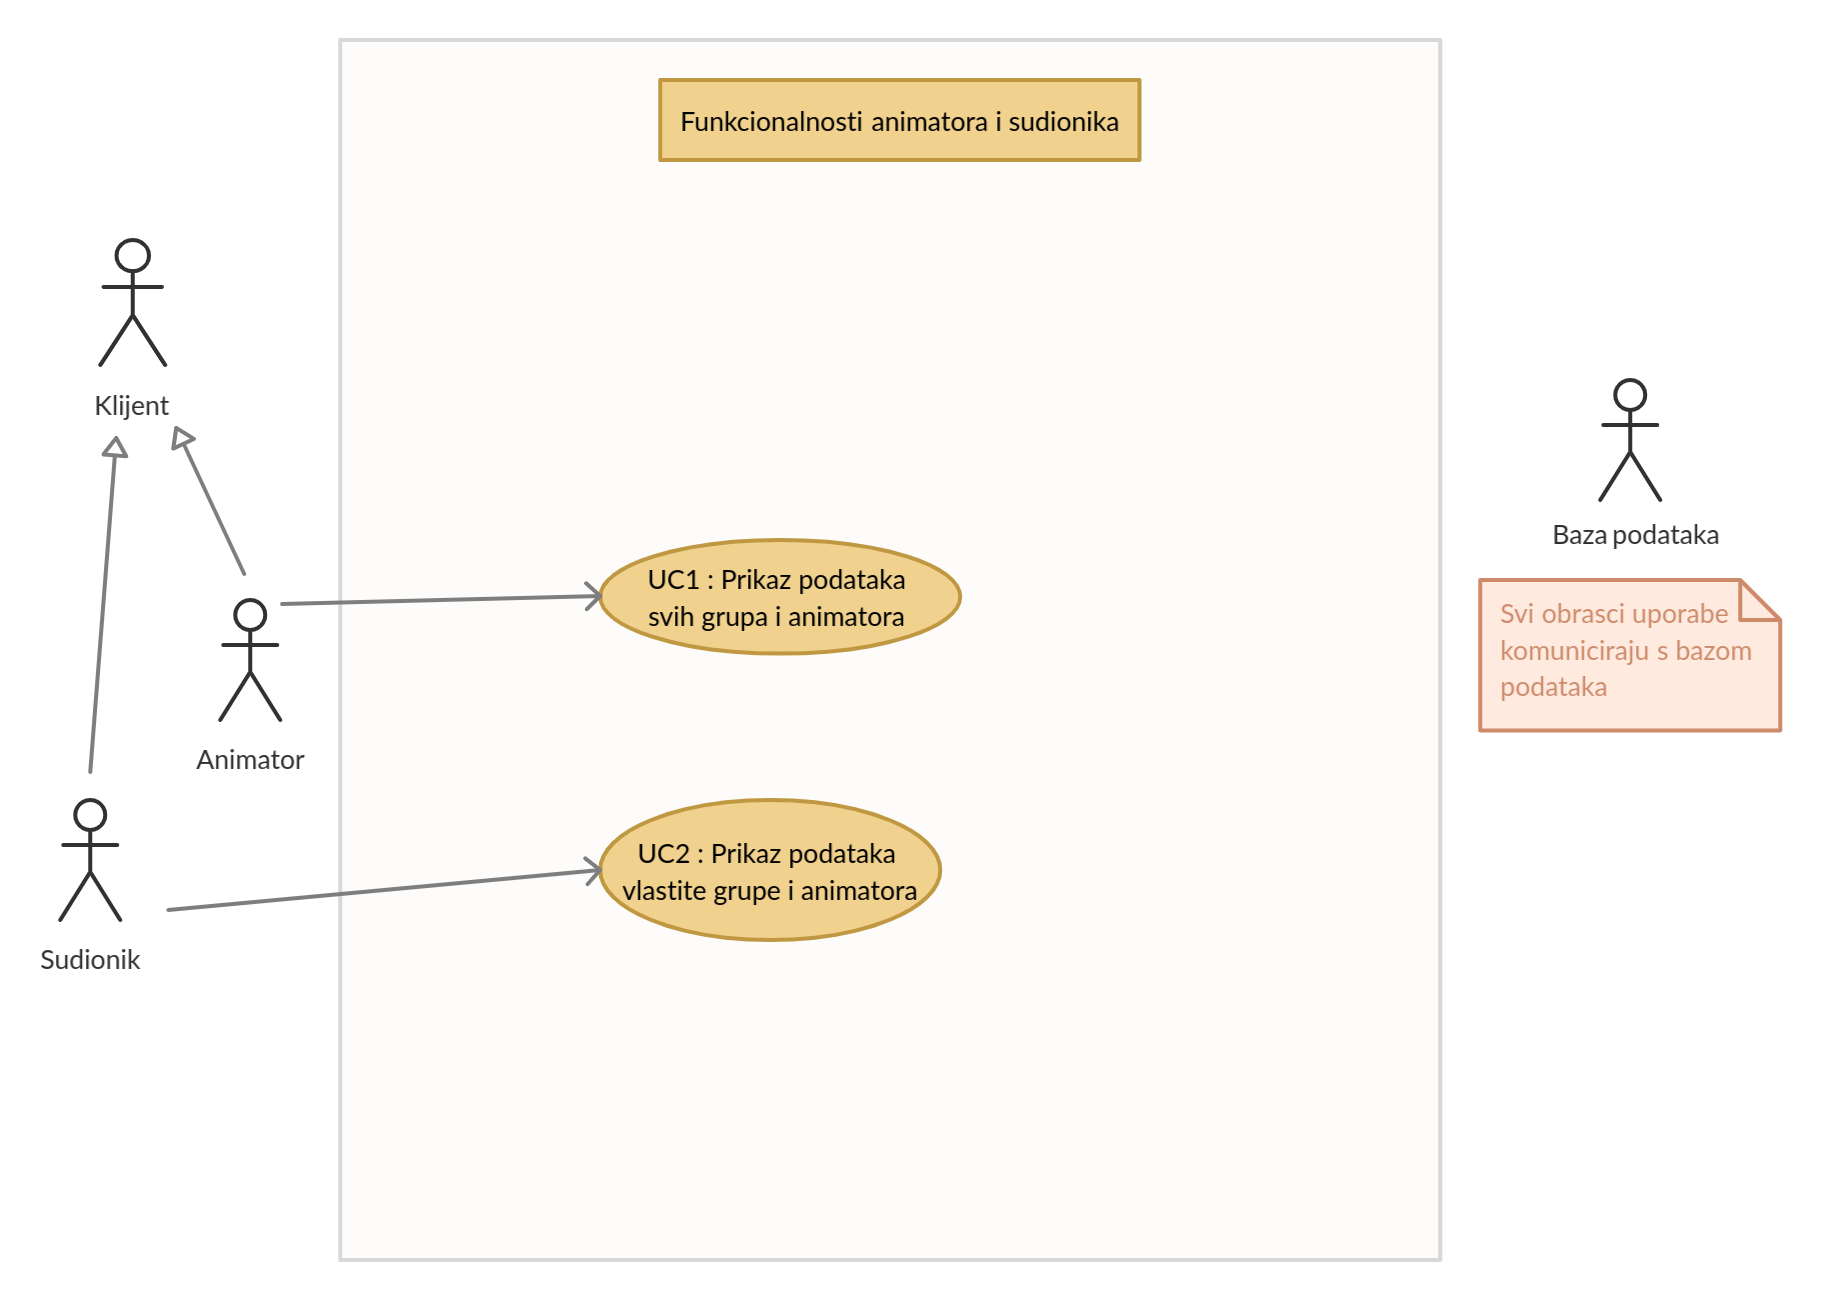
\includegraphics[scale=0.26]{dijagrami/Animator i sudionik.jpg} %veličina slike u odnosu na originalnu datoteku i pozicija slike
	\centering
	\caption{Dijagram obrasca uporabe animator-sudionik.}
	\label{fig:promjene}
\end{figure}

\pagebreak

\begin{figure}[H]
	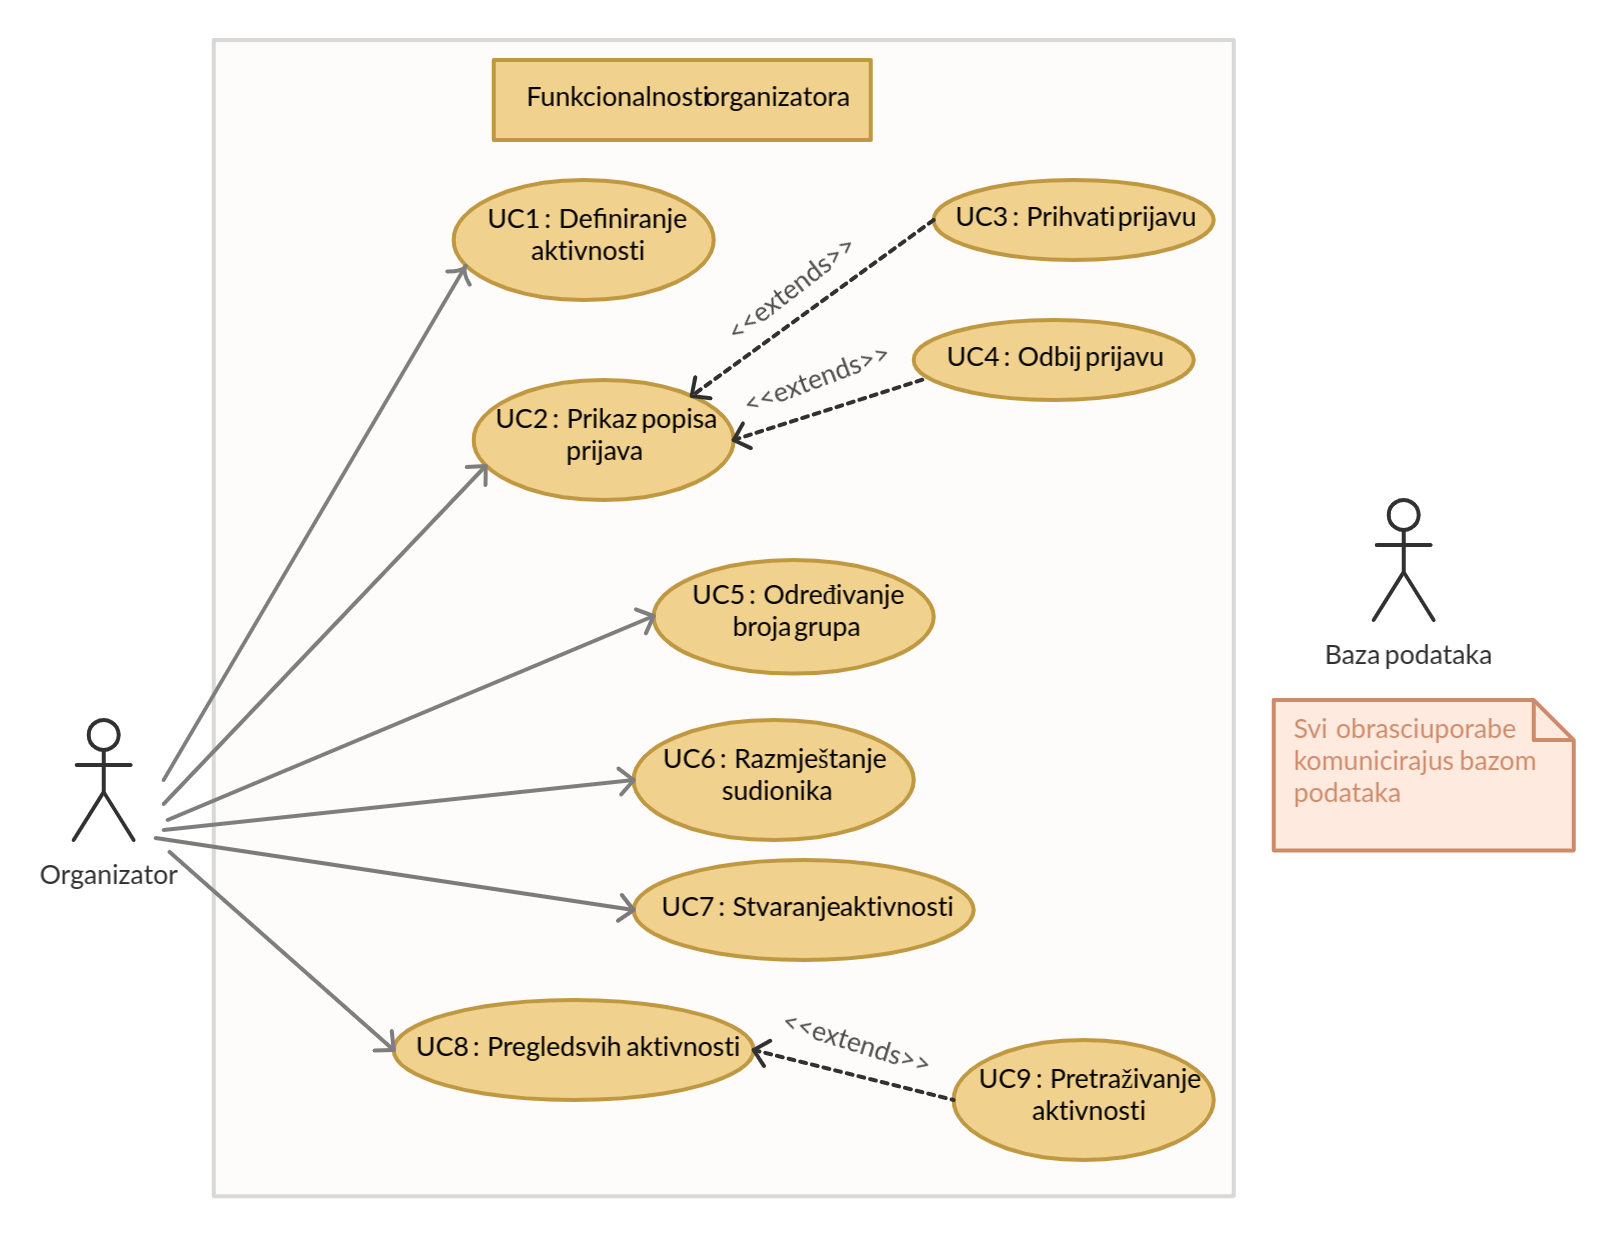
\includegraphics[scale=0.26]{dijagrami/Organizator.jpg} %veličina slike u odnosu na originalnu datoteku i pozicija slike
	\centering
	\caption{Dijagram obrasca uporabe organizatora.}
	\label{fig:promjene}
\end{figure}

\pagebreak

\subsection{Sekvencijski dijagrami}

\textbf{Obrazac uporabe UC2 - Registarcija}

Neregistrirani korisnik odabire opciju za registraciju u određena polja
upisuje osobne podatke kao što su ime, prezime, E-mail te datum rođenja.
Zatim aplikacija provjerava ispravnost unesenih podataka te u slučaju
neispravnih podataka obavještava korisnika. Ako su podaci ispravni unose
se u bazu podataka i ukoliko je korisnik primljen u kamp na E-mail dobiva
personalizirani link na kojem će unijeti svoju lozinku po vlastitom izboru.


\begin{figure}[H]
	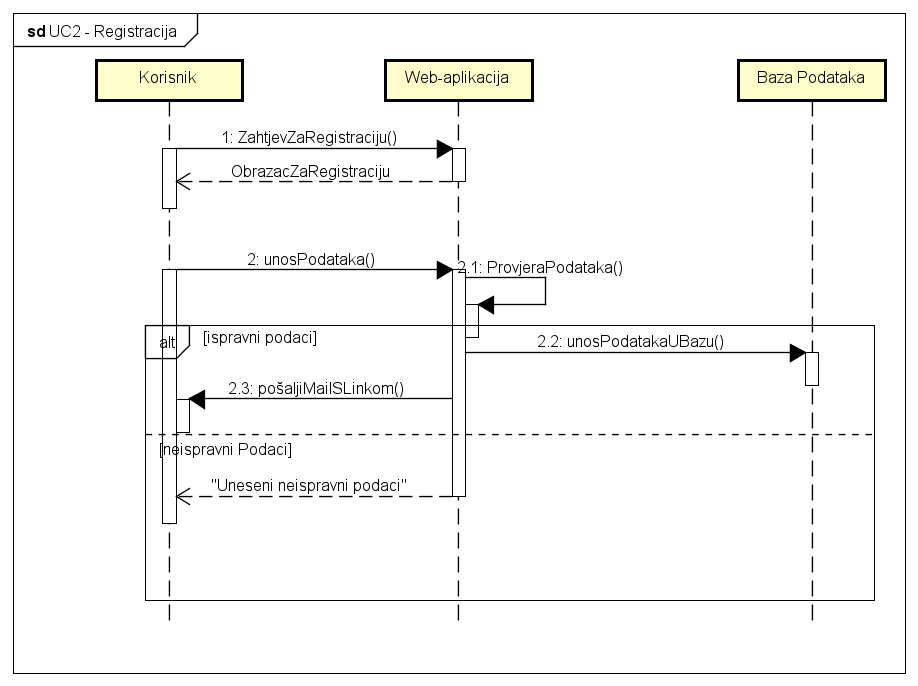
\includegraphics[scale=0.5]{dijagrami/UC2 - Registracija.png} %veličina slike u odnosu na originalnu datoteku i pozicija slike
	\centering
	\caption{Sekvencijski dijagram za UC2}
	\label{fig:promjene}
\end{figure}

\pagebreak

\textbf{Obrazac uporabe UC5 - Prijava u sustav}

Neprijavljeni korisnik šalje zahtjev za prijavu u kojem unosi
svoje korisničko ime i izabranu loznku. Web-aplikacija provjerava
ispravnost podataka tako da provjeri postoji li u bazi podataka
predano korisničko ime, te ako postoji, je li tom korisničkom imenu pridjeljena upisana lozinka. U slučaju uspješne prijave
neprijavljeni korisnik dobije ovlasti prijavljenog korisnika. U slučaju krivog unosa podataka korisnik dobije primjereni odgovor

\begin{figure}[H]
	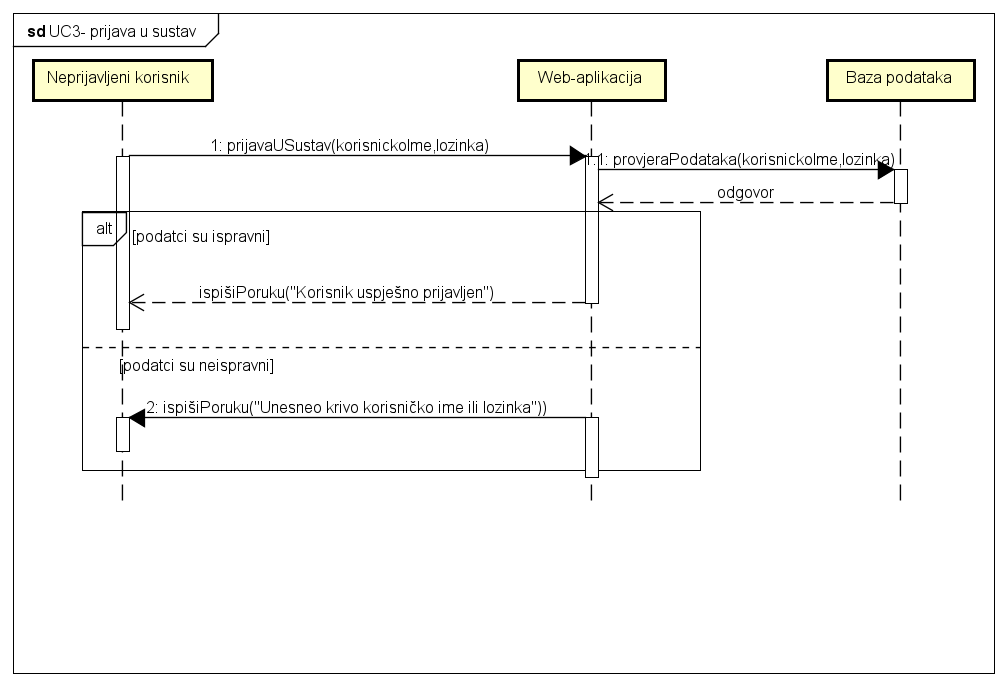
\includegraphics[scale=0.6]{dijagrami/UC3- prijava u sustav.png} %veličina slike u odnosu na originalnu datoteku i pozicija slike
	\centering
	\caption{Sekvencijski dijagram za UC5}
	\label{fig:promjene}
\end{figure}

\pagebreak







\textbf{Obrazac uporabe UC13 - Definiranje aktivnosti}

Organizator šalje zahtjev za definiranje nove aktivnosti. Ogranizator mora upisati ime aktivnosti, kratki opis, vremensko trajanje i tip aktivnosti. U slučaju da nije upisan bilo koji od podataka, ispisuje se poruka o grešci i organizatora se vraća an sučelje za organizatora. U slučaju da su uneseni svi parametri aktivnosti, nova aktivnost se upisuje u bazu podataka


\begin{figure}[H]
	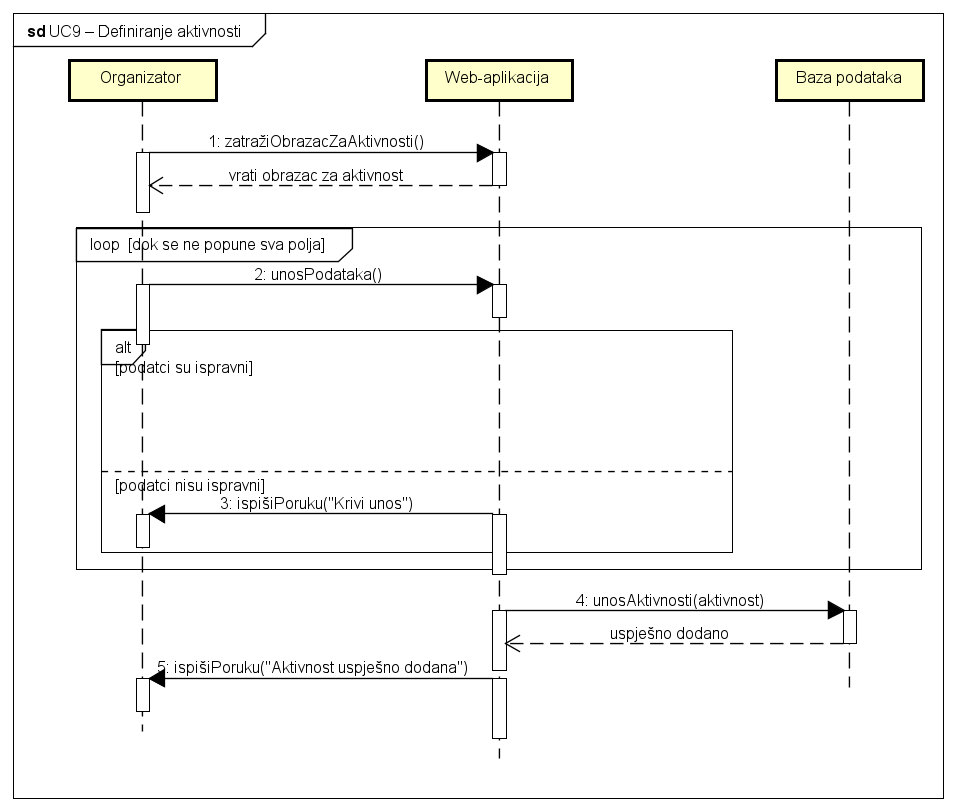
\includegraphics[scale=0.6]{dokumentacija/dijagrami/UC9 ΓÇô Definiranje aktivnosti.png} %veličina slike u odnosu na originalnu datoteku i pozicija slike
	\centering
	\caption{Sekvencijski dijagram za UC13}
	\label{fig:promjene}
\end{figure}

\pagebreak

\textbf{Obrazac uporabe U15 - Određivanje broja grupa}

Nakon što je proces prijava korisnika za kamp završio, organizator vidi popis svih uspješno prijavljenih sudionika.
Organizator u polje za unos podataka unosi broj koliko želi
da bude grupa sudionika. U slučaju unosa tipa podatka koji nije
broj ispisuje se poruka o grešci i omogućava se ponovan unos. U slučaju da je unesen broj grupa koji je veći od ukupnog broja sudionika ispisuje se poruka o grešci i omogućava se ponovan unos. U slučaju da je unesen ispravan broj grupa, formira se taj broj grupi a sudionici se razvrstavaju nasumično.


\begin{figure}[H]
	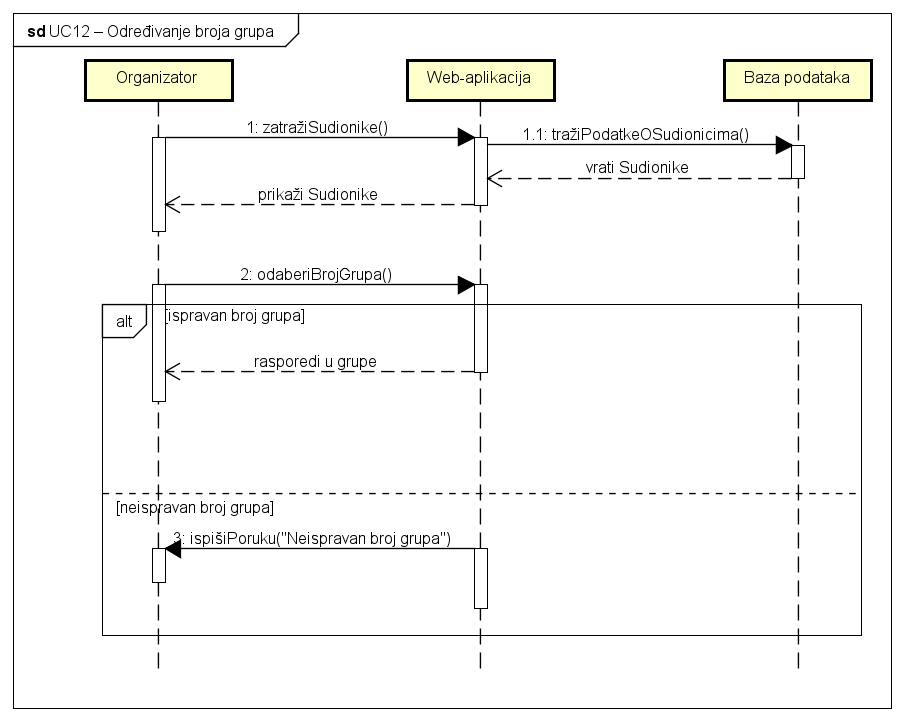
\includegraphics[scale=0.6]{dokumentacija/dijagrami/UC12 Odredivanje broja grupa.png} %veličina slike u odnosu na originalnu datoteku i pozicija slike
	\centering
	\caption{Sekvencijski dijagram za UC15}
	\label{fig:promjene}
\end{figure}
\eject


\section{Ostali zahtjevi}

\begin{itemize}
	\item \text{Sustav treba podržavati rad više korisnika u stvarnom vremenu}
	\item {Sustav treba podržavati hrvatsku abecedu bez gubitka funkcionalnosti}
	\item {Implementacija korisničkog sučelja mora biti korisniku jednostavna i razumljiva za korištenje}
	\item {Sustav treba prikazivati podatke na zathjev korisnika u prihvatljivom vremenu, zahtjevi ne smiju trajati dulje od nekoliko sekundi}
	\item {Sustav bi trebao garantirati točnost podataka koje prikazuje}
	\item {Sustav treba biti temeljen na načelima objektno orijentirane paradigme}
	\item {Ažuriranje sustava i naknadne promjene ne smiju narušavati postojeću funkcionalnost sustava}
	\item {Baza podataka mora biti sigurna i zaštićena od vanjskih utjecaja}
	\item {Korisnikov upit mora biti odgovoren u prihvatljivom vremenu od ne više od par sekundi}
	\item {Neispravno korištenje sustava od korisnika ne smije narušavati funkcionalost sustava}
	\item {Sustavu treba biti omogućen javni pristup preko sigurnog internetskog protokola HTTPS}
\end{itemize}
			 
			 
			 
	
